\documentclass[11pt]{article}
\usepackage[margin=1in]{geometry}
\usepackage{amsmath,amssymb}
\usepackage{booktabs,graphicx}
\usepackage{hyperref}

\newcommand{\eps}{\varepsilon}
\newcommand{\pg}{p_{\mathrm g}}

\title{Resource Cost of a Certified Cosine-Filter State Preparation\\
for the $J_1$--$J_2$ Heisenberg Chain}
\author{}
\date{}

\begin{document}
\maketitle

\begin{abstract}
We report the gate cost of the Stetcu--Baroni--Carlson (SBC) cosine filter as implemented in the
\texttt{j1j2\_filter} pipeline: DMRG front end, low-depth MPS trial circuit, certified filter design,
first- and second-order Trotterisation, and gate counting in an $\{\mathrm{RZZ},R_z,\sqrt{X},X\}$ basis. For the open
spin-$\tfrac12$ $J_1$--$J_2$ chain with $N=4$--$32$, $J_2\in\{0,\,0.2411,\,0.4\}$ and target infidelity
$\eps=10^{-2}$, the certified circuit needs $76$--$24{,}027$ Trotter steps and $1.5\times10^{3}$--$3.6\times10^{6}$
RZZ gates for $N\le 14$, and up to $\sim10^{8}$ RZZ at $N=32$. Certified RZZ count grows as $\sim N^{5}$, steps as
$\sim N^{4}$. The certificate is conservative: the smallest step count that empirically meets $\eps$ is a median
$190\times$ smaller. A second-order (Strang) certificate cuts the certified RZZ count to 3--9\% of the first-order
value for $N=6$--$12$, and an empirical (oracle) design needs only $10^{2}$--$6\times10^{3}$ RZZ for $N\le14$.
\end{abstract}

\section{Pipeline}

The Hamiltonian is $H=\sum_i J_1\,\mathbf S_i\!\cdot\!\mathbf S_{i+1}+J_2\,\mathbf S_i\!\cdot\!\mathbf S_{i+2}$ on an open
chain, and $H_{\mathrm s}$ denotes $H$ shifted and scaled so its spectrum lies in $[0,1]$. The pipeline has five stages.

\begin{enumerate}
\item \textbf{Classical inputs.} DMRG gives $E_0$, the first excited energy $E_1$ (lowest state of any symmetry,
 obtained with a projector penalty), hence the scaled gap $\Delta=(E_1-E_0)/W$. The bandwidth $W$ is the Weyl bound
 $\sum_{\text{bonds}}\lambda_{\max}-E_0$, which equals $E_{\rm top}-E_0$ here. For $N\le14$ exact diagonalisation
 cross-checks these.
\item \textbf{Trial state.} The DMRG MPS is compiled to a one-layer brickwork circuit ($N-1$ two-qubit gates,
 3 non-Clifford RZZ each). Its ground-state weight $\gamma=|\langle g|\psi\rangle|^2$ is $0.31$--$0.99$ over the cases
 studied.
\item \textbf{Filter design.} The ancilla-controlled filter is $F(E)=\prod_i\cos(Et_i+\phi_i)$, built from pulses with
 times $t_i$ and phases $\phi_i$, designed so $\eta=\sup_{[\Delta,1]}|F|/|F(0)|$ is small. Success probability is
 $\pg=\gamma F(0)^2$, and the leakage of excited weight is
 $\ell=(1-\gamma)\eta^2/(\gamma+(1-\gamma)\eta^2)$.
\item \textbf{Trotterisation.} Each pulse $i$ is implemented with $k_i$ steps. At first order the error
 constant $\alpha=\sum_g\|[H_g,\sum_{g'>g}H_{g'}]\|$ is computed exactly from the local Pauli commutators, so the
 filter's operator-norm error is $\epsilon_T=\alpha T^2/(2n)$ with $T=\sum_i t_i$ and $n=\sum_i k_i$. At second
 order (Strang) the per-pulse error is $B_2t_i^3/k_i^2$, with
 $B_2=\tfrac1{12}\sum_a\|[B_a,[B_a,H_a]]\|+\tfrac1{24}\sum_a\|[H_a,[H_a,B_a]]\|$ and $B_a=\sum_{b>a}H_b$
 (Childs et al., PRX 11, 011020, Prop.~16), also evaluated exactly on local supports.
\item \textbf{Count gates.} One Trotter step of one pulse is transpiled once and multiplied by $n$, with one
 $R_z(2\phi_i)$ per pulse. Two compilations are reported: \emph{level 3} (block re-synthesis, 2 RZZ per Pauli term
 per step) and \emph{direct} (4 RZZ per Pauli term, a Clifford ladder around one non-Clifford $R_z$).
\end{enumerate}

\paragraph{Certificate and design rule.} The infidelity of the post-selected state satisfies
\begin{equation}
 1-F\;\le\;\Bigl(\sqrt{\ell}+\epsilon_T/\sqrt{\pg}\Bigr)^2 .
\end{equation}
The pipeline picks the smallest snapped step grid whose right-hand side is $\le\eps$. We call this the
\emph{guaranteed} design. The \emph{empirical} design, the smallest $n$ whose simulated $1-F$ against the exact ground
state is $\le\eps$, is an oracle lower envelope available only for $N\le14$ and is used here only to show how
conservative the certificate is. The proof is in \texttt{CERTIFICATION.tex}.

\paragraph{What is and is not certified.} For $N\le14$ the inputs $\gamma,\Delta$ are checked against ED. For
$N>14$, $\gamma$ is a DMRG-MPS overlap and is \emph{uncertified}, so the guarantee is conditional on DMRG being
accurate. Circuits for $N=16$--$32$ are counted, not simulated.

\section{Results}

All counts are for the success path, $\eps=10^{-2}$, all-to-all connectivity, from
\texttt{results/RESULTS.md}; $T$ is the total filter evolution time in units of $1/J_1$.
Level-3 totals include the trial circuit.

\begin{table}[h]
\centering
\begin{tabular}{rrrrrr}
\toprule
$N$ & $J_2$ & steps $n$ & $T$ ($1/J_1$) & RZZ (level 3) & non-Cliff.\ rot.\ (direct) \\
\midrule
 6 & 0      &    590 &  4.79 & $1.77\times10^{4}$ & $9.4\times10^{3}$ \\
10 & 0      &  3,917 &  7.20 & $2.12\times10^{5}$ & $1.1\times10^{5}$ \\
14 & 0      & 17,822 & 12.76 & $1.39\times10^{6}$ & $7.1\times10^{5}$ \\
\midrule
 6 & 0.2411 &    578 &  3.22 & $3.12\times10^{4}$ & $1.6\times10^{4}$ \\
10 & 0.2411 &  5,777 &  7.38 & $5.89\times10^{5}$ & $3.0\times10^{5}$ \\
14 & 0.2411 & 24,027 & 13.25 & $3.60\times10^{6}$ & $1.8\times10^{6}$ \\
\midrule
 6 & 0.4    &    394 &  2.50 & $2.13\times10^{4}$ & $1.1\times10^{4}$ \\
10 & 0.4    &  2,890 &  3.69 & $2.95\times10^{5}$ & $1.5\times10^{5}$ \\
14 & 0.4    & 10,575 &  7.18 & $1.59\times10^{6}$ & $8.0\times10^{5}$ \\
\bottomrule
\end{tabular}
\caption{Certified (guaranteed) filter designs at $\eps=10^{-2}$ (\texttt{results/tables/dmrg\_guaranteed\_eps0.01\_*.csv}).
Direct compilation uses exactly twice the level-3 filter RZZ count.}
\label{tab:cost}
\end{table}

\paragraph{Scaling.} Fitting $y\propto N^{p}$ over the DMRG points (\texttt{results/tables/scaling\_fits.csv}):

\begin{center}
\begin{tabular}{lccc}
\toprule
 & $J_2=0$ ($N$=6--24) & $0.2411$ (6--28) & $0.4$ (6--32) \\
\midrule
steps $n$        & 3.99 & 4.04 & 3.72 \\
RZZ per step     & 1.10 & 1.14 & 1.13 \\
total RZZ        & 5.08 & 5.18 & 4.86 \\
\bottomrule
\end{tabular}
\end{center}

The $N^{5}$ cost decomposes as $\sim N^{4}$ steps times $\sim N$ RZZ per step (the Pauli-term count is linear in $N$).
The step count itself is driven by $T\propto 1/\Delta$ (fitted $T\sim N^{2.2}$) together with $\alpha T^2/(2\sqrt{\pg})$
and the slowly decaying $\alpha$. At $N=16$--$32$ the counts are $1.6\times10^{4}$--$3.1\times10^{5}$ steps and
$2.4\times10^{6}$--$1.0\times10^{8}$ level-3 RZZ ($4.8\times10^{6}$--$2.0\times10^{8}$ direct).

\begin{figure}[h]
\centering
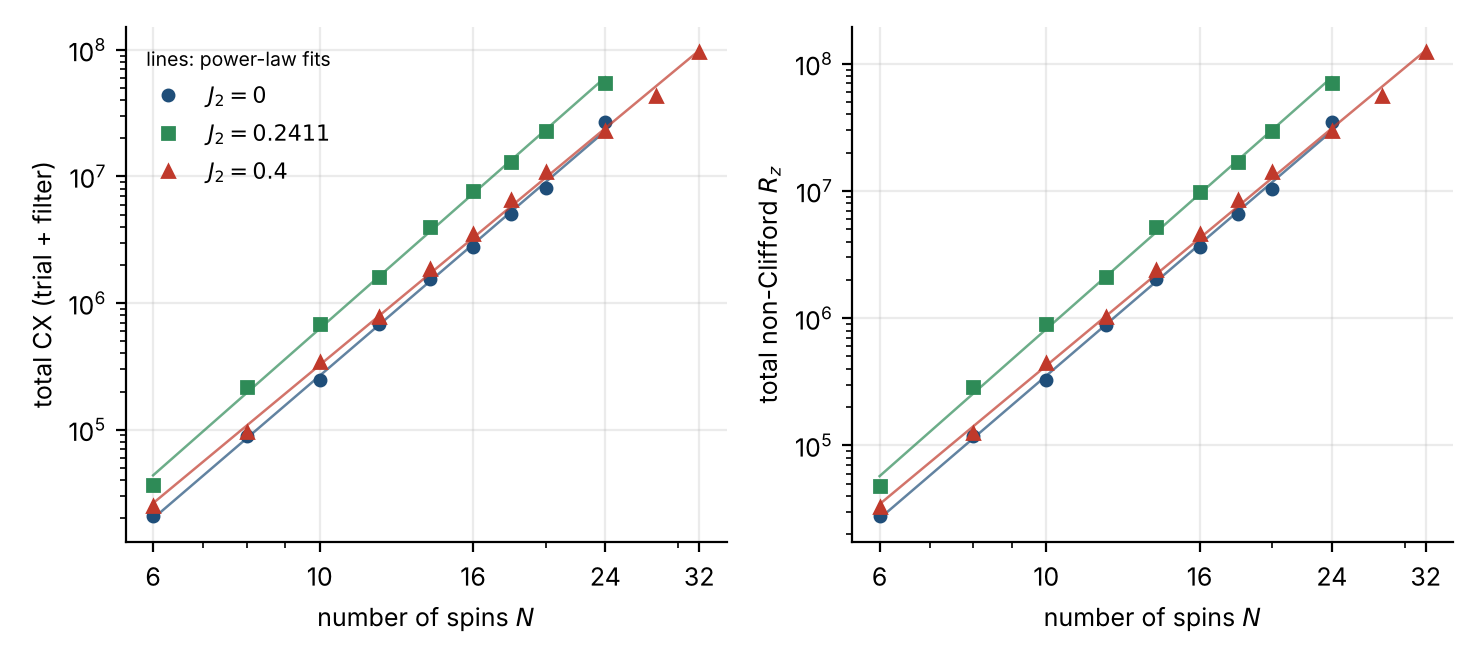
\includegraphics[width=0.8\linewidth]{results/figures_tex/cost_vs_N.png}
\caption{Certified resource cost versus $N$.}
\end{figure}

\paragraph{Conservatism of the certificate.} For the 18 simulated cases ($N\le14$) the bound was never violated.
The empirical design uses $15$--$586\times$ fewer steps (median $190\times$) and $14$--$582\times$ fewer RZZ than the
guaranteed design, almost entirely because the worst-case Trotter term $\epsilon_T$ is loose; the leakage term is
within $\sim1$--$3\times$ of the measured value. The certified numbers above are therefore an upper bound on a
\emph{guaranteed} workflow, not an estimate of the cost a practitioner who simulates would need. Table~\ref{tab:second} (Section~3) gives the first-order empirical designs next to the certified ones; the ratio grows with $N$ at every $J_2$.

\section{Second-order and empirical designs}

\paragraph{Second order.} Keeping the stored pulse times and phases, the second-order design chooses integer
$k_i=\lceil s\,t_i\rceil$ with the smallest $s$ such that $(\sqrt\ell+\sum_i B_2t_i^3/k_i^2/\sqrt{\pg})^2\le\eps$.
The circuits were built with Qiskit's second-order Suzuki--Trotter, transpiled to the RZZ basis and simulated against
ED (\texttt{trotter2/}). This was done for $N=6$--$12$ only, since the commutator evaluation is slow in Python.
Pulse designs were not re-optimised for second order, and the counts are for the filter only (no trial circuit).

\paragraph{Empirical (oracle).} The smallest step count whose \emph{measured} $1-F\le\eps$ against the exact ground
state. It needs the exact state and a simulation, so it is a lower envelope, not something known in advance. For first
order it is available for $N\le14$; for second order, $N\le12$.

\begin{table}[h]
\centering
\small
\begin{tabular}{rr rrrr rrrr}
\toprule
 & & \multicolumn{4}{c}{steps $n$} & \multicolumn{4}{c}{filter RZZ (level 3)} \\
\cmidrule(lr){3-6}\cmidrule(lr){7-10}
$N$ & $J_2$ & cert.\ 1st & cert.\ 2nd & oracle 1st & oracle 2nd & cert.\ 1st & cert.\ 2nd & oracle 1st & oracle 2nd \\
\midrule
 4 & 0      & 85 & -- & 2 & -- & 1,530 & -- & 36 & -- \\
 6 & 0      & 590 & 28 & 5 & 4 & 17,700 & 1,304 & 150 & 224 \\
 8 & 0      & 1,817 & 56 & 11 & 7 & 76,314 & 3,730 & 462 & 545 \\
10 & 0      & 3,917 & 89 & 10 & 7 & 211,518 & 7,679 & 540 & 709 \\
12 & 0      & 8,797 & 168 & 29 & 11 & 580,602 & 17,824 & 1,914 & 1,339 \\
14 & 0      & 17,822 & -- & 39 & -- & 1,390,116 & -- & 3,042 & -- \\
\midrule
 4 & 0.2411 & 94 & -- & 3 & -- & 2,820 & -- & 90 & -- \\
 6 & 0.2411 & 578 & 26 & 6 & 5 & 31,212 & 2,358 & 324 & 489 \\
 8 & 0.2411 & 2,398 & 73 & 11 & 7 & 187,044 & 9,799 & 858 & 1,021 \\
10 & 0.2411 & 5,777 & 125 & 17 & 9 & 589,254 & 22,239 & 1,734 & 1,707 \\
12 & 0.2411 & 10,960 & 187 & 25 & 9 & 1,380,960 & 41,465 & 3,150 & 2,127 \\
14 & 0.2411 & 24,027 & -- & 41 & -- & 3,604,050 & -- & 6,150 & -- \\
\midrule
 4 & 0.4    & 76 & -- & 5 & -- & 2,280 & -- & 150 & -- \\
 6 & 0.4    & 394 & 20 & 6 & 4 & 21,276 & 1,824 & 324 & 400 \\
 8 & 0.4    & 1,059 & 36 & 11 & 5 & 82,602 & 4,848 & 858 & 725 \\
10 & 0.4    & 2,890 & 66 & 16 & 5 & 294,780 & 11,758 & 1,632 & 961 \\
12 & 0.4    & 5,318 & 107 & 26 & 10 & 670,068 & 23,785 & 3,276 & 2,348 \\
14 & 0.4    & 10,575 & -- & 38 & -- & 1,586,250 & -- & 5,700 & -- \\
\bottomrule
\end{tabular}
\caption{Certified and oracle (empirical) designs at first and second order, $\eps=10^{-2}$. First order:
$N=4$--$14$ (\texttt{results/tables/dmrg\_\{guaranteed,empirical\}\_eps0.01\_*.csv}); second order: $N=6$--$12$
(\texttt{trotter2/circuit\_table.md}), ``--'' where not computed. The oracle is the smallest $n$ whose measured $1-F$
against the exact ground state is $\le\eps$. RZZ are filter-only, so the first-order certified entries differ from
Table~\ref{tab:cost}, which includes the trial circuit.}
\label{tab:second}
\end{table}

\begin{itemize}
\item \textbf{Second-order gain.} Over all 12 cases the certified second-order step count is $20$--$59\times$ smaller
 (median $38\times$), growing with $N$. A second-order step costs $1.6$--$1.7\times$ a first-order step, so
 certified RZZ falls to $3.0$--$8.6\%$ of first order (median $4.4\%$; $3.4$--$10.2\%$ with direct compilation).
 The bound held in all 12 simulations, and the Qiskit circuit agrees with the independent simulation to
 $\le10^{-15}$ for $N\le8$.
\item \textbf{Empirical first order} ($N\le14$, $\eps=10^{-2}$): $2$--$41$ steps, $36$--$6{,}150$ filter RZZ, with
 measured $1-F$ between $3\times10^{-3}$ and $10^{-2}$ (\texttt{results/tables/dmrg\_empirical\_eps0.01\_*.csv}).
 This is $15$--$586\times$ below the certified first-order step count.
\item \textbf{Remaining gap.} At second order the certificate is still $5$--$21\times$ the oracle step count
 (first order: $66$--$438\times$ on the same cases), and the gap grows with $N$. The measured second-order state
 error is at most $1\%$ of its bound.
\item \textbf{Oracle caveat.} At small $N$ the second-order oracle is not always cheaper in RZZ than the first-order
 oracle (e.g.\ $N=6$, $J_2=0$: $224$ versus $150$ RZZ), because a second-order step costs more and the first-order
 error can be accidentally small at very few steps. The second-order advantage in the oracle comparison appears at
 larger $N$ (e.g.\ $N=12$, $J_2=0.4$: $2{,}348$ versus $3{,}276$).
\end{itemize}

\section{Caveats}

\begin{itemize}
\item Counts are for the success path; expected cost per accepted run is total$/\pg$ (early abort lowers it).
\item $N=16$--$32$ rely on uncertified DMRG overlaps and are not simulated; no ED check exists there.
\item Level-3 compilation exchanges fewer RZZ for more non-Clifford single-qubit rotations; the per-step non-Clifford
 estimate is accurate to about $\pm20\%$ (\texttt{scripts/audit\_results.py}).
\item Second-order results cover $N\le12$ only, with first-order pulse designs and without the trial circuit. The
 second-order constants are verified numerically (and against the cited proposition), not proved here. The
 $S^2$-projection, symmetric-trial, 2D and field-theory studies are deliberately left out.
\item Gate basis. Native RZZ is cheaper than CNOT here, but the advantage depends on compilation. With direct
 compilation each CNOT maps one-to-one to a Clifford RZZ($\pi/2$), so counts are identical. With level-3
 re-synthesis the RZZ count is $0.86\times$ the CNOT count for the guaranteed designs, since qiskit needs about 2.3 CNOT
 but exactly 2 RZZ per ancilla-controlled Pauli rotation (\texttt{results/tables/cx\_vs\_rzz.csv}). The RZZ basis also
 counts the non-Clifford RZZ($\theta$) rotations in the non-Clifford total.
\item Oracle designs use the exact ground state and are not achievable without it.
\item Open chains only; no hardware connectivity beyond all-to-all (a \emph{line} variant is in \texttt{RESULTS.md}).
\end{itemize}

\paragraph{Reproduction.} \texttt{scripts/run\_results.py} followed by \texttt{scripts/build\_results.py} regenerates
every number from \texttt{pipeline.py}; settings (order, $\eps$, trial layers $=1$) are at the top of that module; the second-order data come from \texttt{trotter2/second\_order\_circuit.py}.

\end{document}
